
%(BEGIN_QUESTION)
% Copyright 2007, Tony R. Kuphaldt, released under the Creative Commons Attribution License (v 1.0)
% This means you may do almost anything with this work of mine, so long as you give me proper credit

Fill a tall glass with water, then take a straw and gently blow air through the straw so that bubbles slowly escape from the straw's end.  Try this with the straw submerged at different levels within the water:

$$\includegraphics[width=15.5cm]{i02955x01.eps}$$

Note how much pressure it takes to blow bubbles out the end of the tube at these different levels by sensing the air pressure within your mouth as you blow (the tension on your cheeks from the air pressure within).

\vskip 10pt

Explain what causes the required air pressure to vary with straw depth, and elaborate on how this principle might be used to measure the level of liquids in a vessel using compressed air and a ``bubble tube.''

\underbar{file i02955}
%(END_QUESTION)





%(BEGIN_ANSWER)


%(END_ANSWER)





%(BEGIN_NOTES)

%INDEX% Measurement, level: bubble tube (bubbler)
%INDEX% Measurement, level: dip tube
%INDEX% Measurement, level: hydrostatic pressure

%(END_NOTES)


